% Self-contained edited transcription of the two supplied PDFs.
% Compile with pdflatex (twice). All four figures are editable TikZ drawings.
% Editorial changes concern prose and presentation; the proofs are not certified.
\documentclass[11pt,letterpaper]{article}
\usepackage[T1]{fontenc}
\usepackage[utf8]{inputenc}
\usepackage{lmodern}
\usepackage[margin=0.85in]{geometry}
\usepackage{amsmath,amssymb,amsthm}
\usepackage{microtype}
\usepackage{tikz}
\usetikzlibrary{arrows.meta}
\usepackage{caption}
\usepackage{fancyhdr}
\usepackage[colorlinks=true,linkcolor=teal,citecolor=teal,urlcolor=teal]{hyperref}
\newcommand{\manuscripttitle}{Connecting the Dots: A Folklore Problem in Real Algebraic Geometry}
\hypersetup{pdftitle={\manuscripttitle}}
\definecolor{curveblue}{HTML}{175F77}
\definecolor{curvered}{HTML}{B74423}
\definecolor{curvegray}{HTML}{718096}
\newcommand{\R}{\mathbb R}
\newcommand{\C}{\mathbb C}
\newcommand{\Vd}{\mathcal V_d}
\newcommand{\norm}[1]{\lVert#1\rVert}
\DeclareMathOperator{\Hess}{Hess}
\newtheorem{theorem}{Theorem}[section]
\newtheorem{lemma}[theorem]{Lemma}
\newtheorem{proposition}[theorem]{Proposition}
\newtheorem*{theoremstar}{Theorem}
\newtheorem*{selectionlemma}{Selection lemma}
\renewcommand{\thesection}{\Roman{part}.\arabic{section}}
\renewcommand{\theHsection}{\arabic{part}.\arabic{section}}
\renewcommand{\theequation}{\Roman{part}.\arabic{equation}}
\renewcommand{\thefigure}{\Roman{part}.\arabic{figure}}
\pagestyle{fancy}
\fancyhf{}
\fancyhead[L]{\small\itshape \manuscripttitle}
\fancyfoot[C]{\thepage}
\setlength{\headheight}{14pt}
\captionsetup{font=small,labelfont=bf}
\setlength{\parskip}{0pt}
\setlength{\emergencystretch}{2em}
\begin{document}
\begin{center}
{\LARGE\bfseries Connecting the Dots:\\[3pt]
A Folklore Problem in Real Algebraic Geometry}\par\medskip
Curated by Paata Ivanisvili and Aleksandr Logunov
\end{center}

\begin{abstract}
Given $n$ points in the Euclidean plane, what is the smallest possible total degree of a nonzero real polynomial in two variables whose zero set has a connected component containing all $n$ points?
This folklore question appears to go back at least to Dmitry Gudkov and Vladimir Rokhlin.
As of November 18, 2026, we did not know whether every set of $n$ points in the Euclidean plane can be contained in a single connected component of the zero set of a nonzero real polynomial of degree $o(n)$, although it has been conjectured that degree $O(\sqrt{n})$ suffices.
On November 19, 2026, ChatGPT (GPT-6.2 Astra), prompted by the curators, generated two texts claiming that both bounds hold.
\end{abstract}

\noindent\textbf{A note from the curators of the Understanding Initiative.} The two texts below were generated entirely by ChatGPT and have not been proof-checked or edited by a human. The text has a positive chance of containing a proof, but is currently hard to read and does not meet any standard of mathematical exposition. We do not claim any credit for the arguments and cannot call ourselves authors.

\smallskip
\noindent The question came up in conversations among Aleksandr Logunov, Ilia Itenberg, and Gadi Kozma in 2023 and has held our interest ever since.
The curators share this text so other curious mathematicians can join them in the pursuit of an answer to and an understanding of this interesting question.

\vspace{-\baselineskip}
\enlargethispage{\baselineskip}
\part{First text: A proof of the weaker sublinear bound}
\label{part:weak}
\begin{abstract}
Let $D(n)$ be the least total degree sufficient to put any $n$ points of the Euclidean plane on a single connected component of the zero set of a nonzero real polynomial. This text gives an argument for $D(n)=o(n)$ by using crossings of interpolating curves to merge groups of prescribed points.
\end{abstract}

Write
\[
Z(P)=\{(x,y)\in\R^2:P(x,y)=0\}.
\]
Taking one line through each prescribed point and a common auxiliary point gives $D(n)\leq n$.
\begin{theoremstar}
We have $D(n)=o(n)$. More precisely, for every fixed integer $d\geq2$, there is a constant $A_d$, independent of $n$, such that
\[
D(n)\leq\frac{d+1}{h}\,n+A_d,\qquad
k=\binom{d+2}{2}-1,\qquad h=\lfloor k/2\rfloor.
\]
\end{theoremstar}
The proof uses a degree-$d$ curve through $k$ selected points. We choose these points so that a path crosses the curve exactly once at each of them. One additional line then joins every component carrying a single selected point. This lets us reduce the number of groups by at least $h$ at a time, at a cost of $d+1$ degrees. Degtyarev and Kharlamov study the corresponding projective interpolation problem in~\cite[\S\S4.6--4.7]{dk2}.

\section{Interpolation in general position}
Let $\Vd$ be the vector space of real polynomials of total degree at most $d$. Its dimension is $N=\binom{d+2}{2}=k+1$. Call a configuration \emph{generic} if evaluations at any $s\leq N$ of its points are linearly independent on $\Vd$, and the unique interpolant through any $k$ of its points, taken up to a nonzero scalar, has a nonsingular real affine zero set. In particular, its gradient is nonzero at every real zero.

\paragraph{Why these conditions are dense.}
Evaluations at all points of the plane span $\Vd^*$, since only the zero polynomial vanishes everywhere. Thus, for each $s\leq N$, an $s$-tuple with independent evaluations exists. Failure of independence is the vanishing of all $s\times s$ minors of the evaluation matrix, a proper algebraic condition.

For smoothness, express the unique interpolant through $k$ points using the signed maximal minors of their $k\times N$ evaluation matrix. The discriminant of its degree-$d$ homogenization is a polynomial in the point coordinates. It is nonzero for some tuple. Indeed, the projective curve $X^d+Y^d-Z^d=0$ is smooth and irreducible over $\C$: two positive-degree components would meet by B\'ezout's theorem. By B\'ezout's theorem again, the polynomials in $\Vd$ vanishing on an entire real affine arc of this curve are precisely the scalar multiples of $x^d+y^d-1$. Evaluations on that arc therefore span a $k$-dimensional space. Choose $k$ independent evaluations there. Their interpolant is the smooth curve just exhibited. Avoiding the finitely many exceptional algebraic sets for all subtuples gives the required dense set of configurations.

\section{One crossing in a pencil of curves}\label{sec:weakcrossing}
A continuous path $\gamma:[0,1]\to\R^2$ \emph{crosses $Z(Q)$ once at $v$} if $Q\circ\gamma$ has exactly one zero $t_0\in(0,1)$, changes sign there, and $\gamma(t_0)=v$.

Let $B$ be a set of $k-1$ points in a generic configuration. Call the other points under consideration \emph{candidates}. The subspace of $\Vd$ vanishing on $B$ has dimension two. Choose a basis $F,G$ with $G$ nonzero at every candidate. This is possible because evaluation at each candidate cuts out a proper line in this two-dimensional space, and finitely many lines cannot cover the space. On $U=\{G\neq0\}$, put $r=F/G$. The polynomial through $B$ and a candidate $v$ is unique up to scale. Take
\[
Q_v=F-r(v)G,\qquad
Q_v(z)=G(z)\bigl(r(z)-r(v)\bigr)\quad(z\in U).
\]
The candidate values $r(v)$ are distinct. Equality at two candidates would give a nonzero polynomial in $\Vd$ vanishing at $k+1=N$ points.

\paragraph{Uniform decomposition.}
There is a number $C_d$ such that $U$ can be partitioned into at most $C_d$ pieces with the following description. On each piece, either $r$ is constant or the piece is homeomorphic to $I\times T$, where $I$ is an interval, $T$ is path connected, and $r$ corresponds to projection onto $I$.

To establish uniformity, let $a,b$ range over coefficient vectors in $\R^N$, and write $F_a,G_b$ for the corresponding polynomials. Apply Hardt's semialgebraic triviality theorem~\cite{hardt} to the continuous semialgebraic map
\[
(a,b,z)\longmapsto\bigl(a,b,F_a(z)/G_b(z)\bigr),\qquad G_b(z)\neq0.
\]
The theorem partitions the target into finitely many semialgebraic parts $Y$. Above each $Y$, there is a homeomorphism with $Y\times T_Y$ under which the map becomes projection onto $Y$. The model fiber $T_Y$ is semialgebraic. The target parts are described by finitely many polynomial sign tests. For fixed $a,b$, these become univariate tests in the last coordinate. The nonzero polynomials have a uniformly bounded total number of roots. These roots and the complementary intervals therefore partition the parameter line into a uniformly bounded number of pieces, each contained in one target part. Restrict the product to each piece and split its model fiber into its finitely many path components. All bounds depend only on $d$.

\paragraph{Local crossing.}
In any ordered list of $m_d=4C_d+1$ candidates, five lie in one piece. Their distinct $r$-values give an increasing or decreasing subsequence of length three. Otherwise, the lengths of the longest increasing and decreasing subsequences ending at each term would give five distinct pairs in $\{1,2\}^2$. The pairs are distinct because, from an earlier term to a later one, one of the two lengths increases.

Write the three candidates as $u<v<w$ in the list order. In their product piece, move the first coordinate strictly monotonically from $r(u)$ through $r(v)$ to $r(w)$. Move the second coordinate along paths through the corresponding three points of $T$. This gives a path from $u$ to $w$ through $v$. Along the path, $G$ has constant nonzero sign, so the displayed identity for $Q_v$ shows that the path crosses $Z(Q_v)$ once at $v$.

\section{Simultaneous crossings}\label{sec:weakselection}
\begin{selectionlemma}
There is an integer $R_d$ such that every generic configuration of at least $R_d$ points contains $k$ points $p_1,\ldots,p_k$ with the following property: a path meets their unique interpolating curve only at these $k$ points, once at each, and changes sides at each crossing.
\end{selectionlemma}
\begin{proof}
Order the configuration arbitrarily. Set $M=\max\{2k+1,k-1+m_d\}$. By the finite Ramsey theorem~\cite{ramsey}, there is an $R_d$ such that every coloring of the $(k+2)$-element subsets of $R_d$ points with at most $2^k$ colors has a homogeneous subset of size $M$. Here, \emph{homogeneous} means that all its $(k+2)$-element subsets have the same color.

To define the color of $z_1<\cdots<z_{k+2}$, record $k$ yes-or-no answers. For position $j$, take $u=z_j$, $v=z_{j+1}$, and $w=z_{j+2}$, and let $B$ consist of the other $k-1$ points. Record ``yes'' if a path from $u$ to $w$ crosses the interpolant through $B\cup\{v\}$ once at $v$. This property depends only on the tuple. Let $H$ be a homogeneous subset of size $M$ for this coloring.

Every entry of the common color is ``yes.'' To see this, fix $j$. For $B$, take the first $j-1$ and the last $k-j$ elements of $H$. At least $m_d$ elements remain in the intervening gap. The local crossing result in Section~\ref{sec:weakcrossing} gives a successful triple in that gap for this fixed $B$. In the resulting $(k+2)$-tuple, the triple starts at position $j$. Homogeneity therefore gives ``yes'' at position $j$ for every such tuple in $H$.

Take $2k+1$ elements of $H$ in the order
\[
w_0<p_1<w_1<p_2<\cdots<w_{k-1}<p_k<w_k.
\]
For each $i$, use the triple $w_{i-1},p_i,w_i$ together with all $p_j$ for $j\neq i$. It occupies three consecutive positions in this tuple, so the corresponding answer is ``yes.'' Each time, the interpolant is the same polynomial $Q$ up to scale, because the conditions are precisely $Q(p_1)=\cdots=Q(p_k)=0$. The path segments share their successive endpoints $w_i$. Concatenating them gives the required path, and smoothness of $Z(Q)$ makes the sign change a crossing between its two local sides.
\end{proof}

\section{Joining the singly marked components}\label{sec:weakjoining}
Every component of $Z(Q)$ is a closed embedded one-dimensional manifold without boundary. It is a circle or a properly embedded copy of $\R$. Either separates the plane into two sides by the Jordan curve theorem. For a proper line, apply the theorem after adding the point at infinity to both the line and the plane.

If a component contains exactly one $p_i$, the path crosses that component once and never returns to it. Its endpoints $w_0,w_k$ therefore lie on opposite sides of the component. The segment $[w_0,w_k]$ must meet it. Thus the single line $L=0$ through the endpoints meets every singly marked component.

The polynomial $QL$ has degree at most $d+1$. Its zero set contains the $k$ selected points in at most $\lceil k/2\rceil$ components. Indeed, if no component of $Z(Q)$ carries a single mark, at most $\lfloor k/2\rfloor$ components carry marks. If $s\geq1$ components carry one mark each, the line joins all $s$ of them. There are then at most
\[
1+\lfloor(k-s)/2\rfloor\leq\lceil k/2\rceil
\]
marked components.

\section{The degree bound}
\paragraph{Iteration.}
Let $S$ be the full generic configuration. Start with $P=1$, and group the points of $S$ by the connected components of $Z(P)\cup S$. Initially, each point is a group. Whenever at least $R_d$ groups remain, take one original point from each group as its representative. The representatives inherit genericity. Apply Sections~\ref{sec:weakselection}--\ref{sec:weakjoining} to them and replace $P$ by $PQL$. The zero set grows by union with $Z(QL)$, so groups can only merge. The $k$ selected groups now occupy at most $\lceil k/2\rceil$ groups. Their number has dropped by at least $k-\lceil k/2\rceil=h$.

There are at most $\lfloor n/h\rfloor$ such steps. Once fewer than $R_d$ groups remain, choose a common point outside $S$ and add one line through it and a representative of each group, multiplying the line equations into $P$. These lines join all the groups. An original point still outside the preceding zero set was isolated in $Z(P)\cup S$ and hence was its own representative. Thus all points now belong to the actual zero set, in one component. The resulting nonzero product has degree at most
\[
D_0=(d+1)\lfloor n/h\rfloor+R_d.
\]

\paragraph{Arbitrary configurations.}
Approximate the given labeled points by generic configurations $S_j$ in the interior of one fixed closed disk $B_R$ centered at the origin. For each $j$, take a polynomial $P_j$ of degree at most $D_0$ and a connected component $C_j$ of $Z(P_j)$ containing $S_j$. Normalize the monomial coefficient vector of $P_j$ to Euclidean norm one. A subsequence converges to the coefficient vector of a nonzero polynomial $P_*$, so $P_j\to P_*$ uniformly on $B_R$.

Let $\rho$ be radial retraction onto $B_R$, fixing the disk. Put $b(x,y)=x^2+y^2-R^2$. The compact connected sets
\[
K_j=\overline{\rho(C_j)}
\]
contain $S_j$ and lie in $Z(bP_j)$, since points outside the disk are sent to its boundary and $Z(bP_j)$ is closed. The space of nonempty compact subsets of $B_R$ is compact in the Hausdorff metric. Pass to a subsequence with limit $K$. It is connected: a separation into two disjoint nonempty compact sets would give disjoint neighborhoods whose union contains $K_j$ and which both meet $K_j$ for all sufficiently large $j$. Each prescribed point belongs to $K$. For $z\in K$, choose $z_j\in K_j$ tending to $z$. Uniform convergence and $b(z_j)P_j(z_j)=0$ give $b(z)P_*(z)=0$. Hence $K\subset Z(bP_*)$.

The polynomial $bP_*$ is nonzero and has degree at most $D_0+2$, so the claimed bound holds with $A_d=R_d+2$. For each fixed $d$, we obtain
\[
0\leq\limsup_{n\to\infty}\frac{D(n)}n\leq\frac{d+1}{h}.
\]
Since $k=d(d+3)/2$ and $h=\lfloor k/2\rfloor$, the last ratio is asymptotic to $4/d$. Letting $d\to\infty$ gives $D(n)/n\to0$.

\begin{thebibliography}{9}
\bibitem{hardt} R. M. Hardt, \emph{Semi-algebraic local-triviality in semi-algebraic mappings}, American Journal of Mathematics \textbf{102} (1980), 291--302.
\bibitem{ramsey} F. P. Ramsey, \emph{On a problem of formal logic}, Proceedings of the London Mathematical Society (2) \textbf{30} (1930), 264--286.
\bibitem{dk2} A. Degtyarev and V. Kharlamov, \emph{Topological properties of real algebraic varieties: du c\^ot\'e de chez Rokhlin}, Russian Mathematical Surveys \textbf{55} (2000), 735--814. \href{https://arxiv.org/abs/math/0004134}{arXiv:math/0004134}.
\end{thebibliography}

\clearpage
\part{Second text: A square-root degree bound}
\label{part:strong}
\setcounter{section}{0}
\setcounter{equation}{0}
\setcounter{figure}{0}
\begin{abstract}
Let $D(n)$ be the least degree sufficient to place any $n$ prescribed points in the real plane on one connected component of a polynomial zero set. We prove that $D(n)=\Theta(\sqrt n)$, with $D(n)\leq64\sqrt n+2$ for every $n$ and $\limsup_{n\to\infty}D(n)/\sqrt n<44.23$. The upper bound rests on a property of a pencil of degree-$d$ curves. Consider its rational parameter $F/G$ on a finite sample at which its values are distinct and its gradients are nonzero. For all but $O(d^2)$ sample points $v$, a path between two other sample points crosses the level of $v$ exactly once, at $v$. If the fiber is smooth, its component through $v$ separates the two endpoints. Averaging over interpolation conditions allows us to remove on the order of $d^2$ prescribed points and restore them at a cost of $d$ degrees.
\end{abstract}
\noindent\textit{Remark.} This AI-generated text presents a proposed proof and requires human verification.

\section{Introduction}
Write $Z(P)=\{z\in\R^2:P(z)=0\}$ for the real affine zero set of a nonzero polynomial $P\in\R[x,y]$. All connected components are taken in the ordinary Euclidean topology. Let $D(n)$ be the smallest integer $D$ such that every set of $n$ points in $\R^2$ lies in a single component of $Z(P)$ for some $P$ of total degree at most $D$. Reducible polynomials are allowed. Multiplying polynomials takes the union of their zero sets; we use this operation to connect the curves we construct.
\begin{theorem}\label{thm:strong}
For every $n\geq1$,
\begin{equation}\label{eq:main}
\left\lfloor\frac{\sqrt{8n+1}-1}{2}\right\rfloor
\leq D(n)\leq64\sqrt n+2.
\end{equation}
In addition, $\displaystyle\limsup_{n\to\infty}\frac{D(n)}{\sqrt n}<44.23$.
\end{theorem}
Ordinary interpolation explains the scale in \eqref{eq:main}. The space of polynomials of degree at most $d$ has dimension $\binom{d+2}{2}$. Any set of fewer than this many points therefore lies in the zero set of a nonzero polynomial of degree at most $d$. This dimension count gives no information about which components contain the points. We use a pair of additional points to control the component through a prescribed point $v$. If that component separates the pair, every connected set containing the pair must meet it. Section~\ref{sec:removal} shows how to find such pairs for many points at once. With $m$ points remaining, take $d$ proportional to $\sqrt m$. A single degree-$d$ curve then accounts for a fixed fraction of the points. Iteration yields a geometric decrease in $m$, and the degrees sum to $O(\sqrt n)$.

\paragraph{The projective problem.}
Degtyarev and Kharlamov~\cite[\S\S4.6--4.7]{dk1} define $c'(d)$ as the largest number of arbitrary points in $\R\mathrm P^2$ guaranteed to lie on one real component of a degree-$d$ projective curve. Their Propositions~4.7.2 and~4.7.4 give
\[
3d-1\leq c'(d)\leq\frac38d^2+O(d).
\]
Every finite projective configuration fits in an affine chart. Homogenizing an affine interpolant preserves the connected subset containing the points. Adding distinct real lines, if necessary, raises its degree to exactly $d$. Consequently, $n\leq c'(D(n))$. Their upper bound therefore also gives
\[
\liminf_{n\to\infty}\frac{D(n)}{\sqrt n}\geq\sqrt{8/3}.
\]
Conversely, \eqref{eq:main} gives $c'(d)\gtrsim d^2$. Thus the order of growth is sharp in both formulations.

\section{Interpolation and planar separation}
For $d\geq1$, put
\begin{equation}\label{eq:dimension}
\Vd=\R[x,y]_{\leq d},\qquad
N_d=\dim\Vd=\binom{d+2}{2},\qquad
k_d=N_d-1=\frac{d(d+3)}2.
\end{equation}
The evaluations $P\mapsto P(z)$, $z\in\R^2$, span $\Vd^*$, since a polynomial vanishing everywhere is zero. Thus $N_d$ independent evaluations can be chosen. If $N_d\leq n$, adjoining arbitrary further distinct points gives an $n$-point set on which no nonzero member of $\Vd$ vanishes. Hence $D(n)$ is at least the smallest $d$ with $N_d>n$, which gives the lower bound in \eqref{eq:main}.

\begin{lemma}[Generic interpolation]\label{lem:generic}
For any fixed $n$ and finite list of positive degrees $d$, there is a dense set of labeled $n$-point configurations with the following properties at every listed degree. Each subset of at most $N_d$ points gives independent evaluations on $\Vd$. Each $k_d$-point subset determines, up to a nonzero scalar, a unique nonzero member of $\Vd$ whose gradient is nonzero at every real zero.
\end{lemma}
\begin{proof}
Independence is equivalent to the nonvanishing of at least one evaluation minor, and the spanning argument shows that the exceptional locus is proper. For $k_d=N_d-1$ independent rows, the signed maximal minors give a kernel vector. The discriminant of the degree-$d$ homogenization of the corresponding polynomial is therefore a polynomial in the point coordinates.

For $d\geq2$, consider the smooth complex projective curve $X^d+Y^d-Z^d=0$. It is irreducible: positive-degree factors would meet by B\'ezout's theorem~\cite{fulton} and produce a singular point. Its real affine locus contains a smooth arc. By B\'ezout's theorem, any member of $\Vd$ vanishing on that arc is a scalar multiple of $x^d+y^d-1$. Evaluations on the arc have rank $k_d$, so $k_d$ points on it determine this curve. The discriminant therefore takes a nonzero value. For $d=1$, the assertion follows from the line through two distinct points. Avoiding the finitely many proper algebraic exceptional sets over all listed degrees and subsets proves the claim.
\end{proof}

\begin{lemma}[Restoring a point by separation]\label{lem:separation}
Let $Z(Q)$ be nonsingular in $\R^2$. Suppose a continuous path from $u$ to $w$ meets $Z(Q)$ at exactly one parameter value, at $v$, and $Q$ changes sign there. Every connected set containing $u$ and $w$ meets the component $C_v$ of $Z(Q)$ containing $v$.
\end{lemma}
\begin{proof}
A component of the closed, smooth one-dimensional manifold $Z(Q)$ is an embedded circle or a properly embedded copy of $\R$. Each separates the plane by the Jordan curve theorem. For a proper line, its one-point compactification is a Jordan curve in the sphere. The implicit function theorem identifies the two local sides at $v$ with the two signs of $Q$. The path crosses from one side of $C_v$ to the other at $v$ and never meets $C_v$ again. Thus $u$ and $w$ lie in different components of its complement.
\end{proof}

\begin{figure}[htbp]
\centering
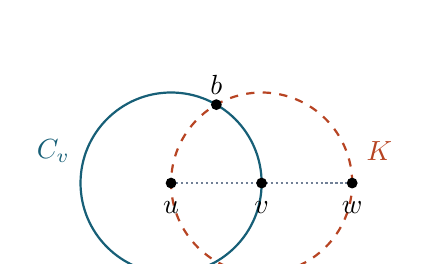
\begin{tikzpicture}[scale=1.15]
\draw[curveblue,thick] (0,0) circle (1);
\draw[curvered,thick,dashed] (1,0) circle (1);
\draw[curvegray,densely dotted,thick] (0,0)--(2,0);
\foreach \x/\lab in {0/u,1/v,2/w}{\fill (\x,0) circle (1.7pt) node[below=3pt] {$\lab$};}
\fill (0.5,0.8660254) circle (1.7pt) node[above] {$b$};
\node[curveblue] at (-1.3,0.35) {$C_v$};
\node[curvered] at (2.3,0.35) {$K$};
\end{tikzpicture}
\caption{The two unit circles $C_v=\{x^2+y^2=1\}$ and $K=\{(x-1)^2+y^2=1\}$. The segment from $u=(0,0)$ to $w=(2,0)$ crosses $C_v$ only at $v=(1,0)$. The curve $K$ joins $u$ and $w$ and meets $C_v$ at $(1/2,\pm\sqrt3/2)$.}
\end{figure}

\section{Exceptional points in a rational pencil}
Fix $F,G\in\Vd$, with $G\not\equiv0$. On the open set $U=\{G\neq0\}$, the function $r=F/G$ parametrizes the pencil $F-tG=0$. We first study a finite sample for an arbitrary such function.
\begin{lemma}[Two witnesses]\label{lem:witnesses}
Let $V\subset U$ be a finite nonempty set. Suppose the values $r(v)$, $v\in V$, are pairwise distinct and $\nabla r(v)\neq0$ for every $v\in V$. With at most $b_d=2(3d+1)^2$ exceptions, each $v\in V$ admits points $u,w\in V\setminus\{v\}$ and a continuous path $\gamma:[0,1]\to U$ from $u$ to $w$ with the following property: for some $s\in(0,1)$, $\gamma(s)=v$, and
\[
r(\gamma(t))<r(v)\quad(0\leq t<s),\qquad
r(\gamma(t))>r(v)\quad(s<t\leq1).
\]
\end{lemma}
\begin{proof}
Write $t_v=r(v)$. Near $v$, one can use $r-t_v$ as a smooth coordinate. Inside a sufficiently small coordinate rectangle, the region where $r<t_v$ is connected and accumulates at $v$. Let $W_v$ be the component of $\{z\in U:r(z)<t_v\}$ containing this local lower side. Call $v$ \emph{exceptional from below} if $W_v\cap V=\varnothing$.

\emph{Disjointness.} The regions $W_v$ corresponding to points exceptional from below are pairwise disjoint. Indeed, suppose $t_v<t_w$ and $W_v\cap W_w\neq\varnothing$. Since $v\in\overline{W_v}$, the set $W_v\cup\{v\}$ is connected. It lies in $\{r<t_w\}$ and meets its component $W_w$, so it is contained in $W_w$. Then $v\in W_w\cap V$, a contradiction.

\begin{figure}[htbp]
\centering
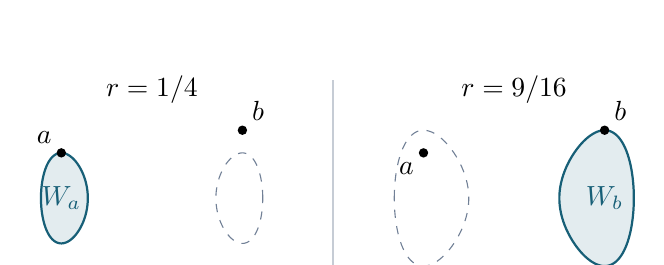
\begin{tikzpicture}[x=1.15cm,y=1.15cm]
\begin{scope}
\node at (0,1.2) {$r=1/4$};
\draw[curveblue,thick,fill=curveblue!12] plot[domain=0:360,samples=100] ({-sqrt(1+0.5*cos(\x))},{0.5*sin(\x)});
\draw[curvegray,dashed] plot[domain=0:360,samples=100] ({sqrt(1+0.5*cos(\x))},{0.5*sin(\x)});
\fill (-1,0.5) circle (1.7pt) node[above left] {$a$};
\fill (1,0.75) circle (1.7pt) node[above right] {$b$};
\node[curveblue] at (-1,0) {$W_a$};
\end{scope}
\draw[curvegray!40] (2,-0.85)--(2,1.3);
\begin{scope}[xshift=4.6cm]
\node at (0,1.2) {$r=9/16$};
\draw[curvegray,dashed] plot[domain=0:360,samples=100] ({-sqrt(1+0.75*cos(\x))},{0.75*sin(\x)});
\draw[curveblue,thick,fill=curveblue!12] plot[domain=0:360,samples=100] ({sqrt(1+0.75*cos(\x))},{0.75*sin(\x)});
\fill (-1,0.5) circle (1.7pt) node[below left] {$a$};
\fill (1,0.75) circle (1.7pt) node[above right] {$b$};
\node[curveblue] at (1,0) {$W_b$};
\end{scope}
\end{tikzpicture}
\caption{For $r=(x^2-1)^2+y^2$, take $V=\{a,b\}$, with $a=(-1,1/2)$ and $b=(1,3/4)$. At $t_a=1/4$, the lower side at $a$ lies in the left lobe. At $t_b=9/16$, the lower side at $b$ lies in the right lobe. Both shaded components are sample-free, although $a$ belongs to the other lobe at the second level. The lobes remain disjoint because $r(0,y)\geq1$.}
\end{figure}

\emph{Forcing a critical point in each region.} Fix $T<\min_{v\in V}t_v$. For each point exceptional from below, choose $z_v\in W_v$ close enough to $v$ that $T<r(z_v)<t_v$. For $\varepsilon>0$ and $c\in\R^2$, set
\begin{equation}\label{eq:barrier}
H_c(z)=(r(z)-T)^2+\frac{\varepsilon}{G(z)^2}+\varepsilon\norm{z-c}^2,
\qquad z\in U.
\end{equation}
Choose a single $\varepsilon>0$ so small that $H_c(z_v)<(t_v-T)^2$ simultaneously for all chosen $z_v$ and all $\norm c\leq1$. This is possible because the inequalities are strict at $\varepsilon=0$, there are finitely many test points, and $\norm{z_v-c}\leq\norm{z_v}+1$.

Every sublevel set of $H_c$ is compact in $U$. Indeed, the last term in \eqref{eq:barrier} bounds $\norm z$, while the middle term bounds $|G(z)|$ away from zero. On the boundary of $W_v$ relative to $U$, one has $r=t_v$. This follows from continuity and the fact that the components of the open set $\{r<t_v\}$ are both open and relatively closed in that set. Thus $H_c\geq(t_v-T)^2$ on this boundary. Compactness of the sublevel set through $z_v$ gives a minimum on the relative closure of $W_v$, and the strict inequality at $z_v$ places this minimum in $W_v$. By disjointness, different exceptional points force different critical points of the same function $H_c$.

\begin{figure}[htbp]
\centering
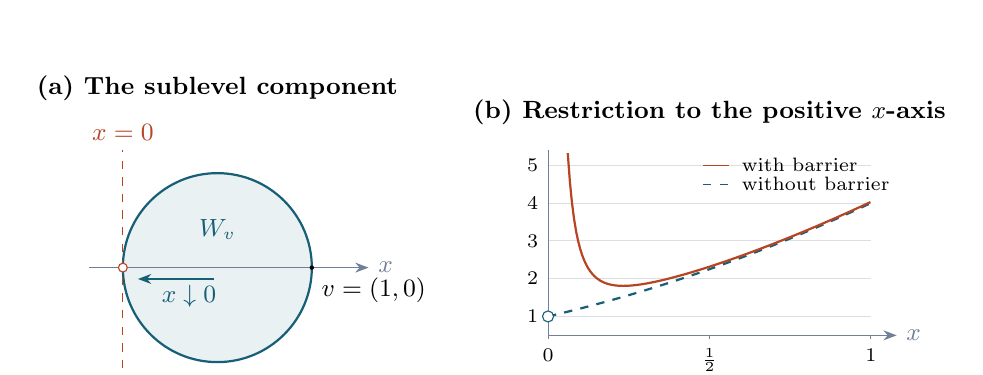
\begin{tikzpicture}[font=\small]
\begin{scope}[x=2.4cm,y=2.4cm]
\node[font=\small\bfseries] at (0.5,0.95) {(a) The sublevel component};
\draw[curveblue,thick,fill=curveblue!9] (0.5,0) circle (0.5);
\draw[curvered,dashed] (0,-0.62)--(0,0.62) node[above] {$x=0$};
\draw[-{Stealth},curvegray] (-0.18,0)--(1.3,0) node[right] {$x$};
\fill (1,0) circle (0.8pt) node[below right] {$v=(1,0)$};
\draw[curvered,fill=white] (0,0) circle (1.6pt);
\node[curveblue] at (0.5,0.2) {$W_v$};
\draw[-{Stealth},curveblue] (0.48,-0.06)--(0.08,-0.06);
\node[curveblue] at (0.35,-0.15) {$x\downarrow0$};
\end{scope}
\begin{scope}[xshift=5.4cm,yshift=-1.1cm,x=4.1cm,y=0.48cm]
\node[font=\small\bfseries] at (0.5,6.4) {(b) Restriction to the positive $x$-axis};
\foreach \y in {1,2,3,4,5}{\draw[curvegray!25] (0,\y)--(1,\y);\node[left,font=\scriptsize] at (0,\y) {$\y$};}
\draw[-{Stealth},curvegray] (0,0.5)--(1.08,0.5) node[right] {$x$};
\draw[curvegray] (0,0.5)--(0,5.4);
\foreach \x/\lab in {0/0,0.5/{\tfrac12},1/1}{\draw[curvegray] (\x,0.5)--(\x,0.4);\node[below,font=\scriptsize] at (\x,0.4) {$\lab$};}
\draw[curveblue,dashed,thick] plot[domain=0:1,samples=100] (\x,{(\x+1)^2});
\begin{scope}\clip (0,0.5) rectangle (1,5.3);
\draw[curvered,thick] plot[domain=0.055:1,samples=150] (\x,{(\x+1)^2+1/(64*\x^2)+\x^2/64});\end{scope}
\draw[curveblue,fill=white] (0,1) circle (2pt);
\draw[curvered] (0.48,5)--(0.56,5);\node[right,font=\scriptsize] at (0.57,5) {with barrier};
\draw[curveblue,dashed] (0.48,4.5)--(0.56,4.5);\node[right,font=\scriptsize] at (0.57,4.5) {without barrier};
\end{scope}
\end{tikzpicture}
\caption{For $r=(x^2+y^2)/x$, the lower component at $v=(1,0)$ is the open disk $(x-1/2)^2+y^2<1/4$. It approaches the deleted line $x=0$ at the origin. With $T=-1$, the function $(r+1)^2$ has unattained infimum $1$ on this disk. The right panel shows the restriction to $y=0$. For $c=0$ and $\varepsilon=1/64$, the term $\varepsilon/x^2$ sends $H_0$ to infinity at the pole, while $H_0(1/2,0)<4=(t_v-T)^2$.}
\end{figure}

\emph{Counting critical points.} Put $h=(r-T)^2+\varepsilon/G^2$. By Sard's theorem~\cite{sard}, there is a regular value $c$, with $\norm c<1$, of the smooth map
\[
\Phi:U\longrightarrow\R^2,\qquad
\Phi(z)=z+\frac1{2\varepsilon}\nabla h(z).
\]
Since $\nabla H_c=2\varepsilon(\Phi-c)$, all critical points of $H_c$ are nondegenerate. Set $E=F-TG$. Multiplying $\nabla H_c/2$ by $G^3$ gives the polynomial vector
\begin{equation}\label{eq:critical}
EG\nabla E-(E^2+\varepsilon)\nabla G+\varepsilon G^3(z-c).
\end{equation}
Both entries have degree at most $3d+1$. At a critical point, their Jacobian is $(G^3/2)\Hess H_c$, which is invertible. Thus B\'ezout's theorem bounds the number of such common zeros by $(3d+1)^2$. For completeness, a common complex factor cannot vanish at a nonsingular common zero, since the gradients of both entries there would be multiples of its gradient. Cancel the greatest common divisor and apply B\'ezout's theorem to the coprime pair, homogenized to its actual degrees. This bounds all nonsingular real common zeros, regardless of any other common components.

We have bounded the number of exceptions from below by $(3d+1)^2$. Apply the same argument to $-r$ to bound the number of exceptions from above. For a point exceptional on neither side, choose $u$ in the adjacent lower component and $w$ in the adjacent upper component, both in $V$. An open connected subset of $\R^2$ is path connected. Travel from $u$ within the lower component to a short coordinate segment entering $v$ from below, cross $v$ on that segment, and continue within the upper component to $w$. This gives the required path.
\end{proof}

\section{Simultaneous removal and the degree bound}\label{sec:removal}
Fix $d\geq2$, write $k=k_d$, and suppose $S$ is a generic set of $m\geq k+1$ points as in Lemma~\ref{lem:generic}. A pair $(B,v)$, where $B\subset S$, $|B|=k-1$, and $v\in S\setminus B$, determines, up to a nonzero scalar, a unique interpolant $Q\in\Vd$ through $B\cup\{v\}$. Call the pair \emph{good} if a path between two points of $S\setminus(B\cup\{v\})$ meets $Z(Q)$ only at $v$, at a single parameter value where $Q$ changes sign.
\begin{samepage}
\begin{proposition}[One removal step]\label{prop:removal}
There are a subset $S'\subset S$ and a nonzero polynomial $Q\in\Vd$ such that
\begin{equation}\label{eq:removal}
q:=m-|S'|\geq k\left(1-\frac{2(3d+1)^2}{m-k+1}\right).
\end{equation}
If one component of $Z(P')$ contains $S'$, then one component of $Z(P'Q)$ contains $S$.
\end{proposition}
\end{samepage}
\begin{proof}
Fix $B$. The polynomials in $\Vd$ vanishing on $B$ form a two-dimensional linear space. For each $v\in S\setminus B$, the additional condition of vanishing at $v$ cuts out a proper line in this space, by independence of evaluations. Avoid the union of these finitely many lines to choose $G$ nonzero at every candidate $v$. Complete $G$ to a basis $F,G$, put $r=F/G$, and set
\[
Q_v=F-r(v)G,\qquad Q_v(z)=G(z)\bigl(r(z)-r(v)\bigr)\quad(z\in U).
\]
The values $r(v)$ are distinct; otherwise, a nonzero $Q_v$ would vanish at $k+1=N_d$ independent evaluations. Also, $\nabla r(v)=\nabla Q_v(v)/G(v)\neq0$ by genericity. Apply Lemma~\ref{lem:witnesses} to $V=S\setminus B$. Along the resulting path, $G$ has constant nonzero sign, so all but at most $b_d=2(3d+1)^2$ of the pairs $(B,v)$ are good.

Choose a uniformly random $k$-element subset $A\subset S$, and then a uniformly random $v\in A$. The pair $(A\setminus\{v\},v)$ has the same distribution as a uniformly random $(k-1)$-element subset $B$ followed by a uniformly random $v\in S\setminus B$. Indeed,
\[
\binom mk k=\binom m{k-1}(m-k+1).
\]
The probability of failure is at most $b_d/(m-k+1)$. Taking the expected number of good marked points in $A$ gives a set $A$ with at least the number in the right-hand side of \eqref{eq:removal}. Use the same polynomial $Q$ for all of them: the interpolant through $A$.

Delete precisely these good marked points to form $S'$. Both witnesses for each deleted point $v$ belong to $S\setminus A$, so both remain. If $K$ is a component of $Z(P')$ containing $S'$, Lemma~\ref{lem:separation} gives $K\cap C_v\neq\varnothing$ for every deleted point. Hence $K\cup\bigcup_v C_v$ is connected, contains $S$, and is contained in $Z(P'Q)$.
\end{proof}

\paragraph{Choice of degree.}
When $m\geq256$, take $d=\lfloor\sqrt m/8\rfloor$. Then $d\geq2$, $64d^2\leq m<64(d+1)^2$, and
\[
k+2b_d\leq2d^2+4(7d/2)^2=51d^2\leq m.
\]
Inequality~\eqref{eq:removal} therefore removes $q\geq k/2$ points. Writing $m'=m-q$, we obtain
\begin{equation}\label{eq:telescope}
\sqrt m-\sqrt{m'}=\frac q{\sqrt m+\sqrt{m'}}
\geq\frac{d(d+3)}{8\sqrt m}\geq\frac d{64}.
\end{equation}

\paragraph{Iterating the construction.}
Choose the initial $n$-point configuration to be generic simultaneously at all degrees from $1$ through $\max(1,\lfloor\sqrt n/8\rfloor)$. Its subsets inherit all required conditions. Continue removing points until $s<256$ remain. Take one line through each remaining point and a common auxiliary point. Their product has a connected zero set and degree $s\leq16\sqrt s$. Now restore the deleted points in reverse order using Proposition~\ref{prop:removal}. Summing \eqref{eq:telescope} over all stages bounds the total degree by
\[
16\sqrt s+64(\sqrt n-\sqrt s)\leq64\sqrt n.
\]
This proves the upper bound for generic configurations.

\section{Passage to arbitrary configurations}
Affine connections can disappear in a coefficient limit, even with two fixed marked points. The following compactness argument costs two additional degrees.
\begin{lemma}\label{lem:limit}
Suppose a sequence of labeled $n$-point configurations converges coordinatewise to $S$. If each configuration lies on one component of a nonzero polynomial zero set of degree at most $D$, then $S$ lies on one component of such a zero set of degree at most $D+2$.
\end{lemma}
\begin{proof}
Choose a closed disk $B_R=\{\norm z\leq R\}$ containing all configurations in its interior. Write $P_j$ for their polynomials and $K_j\subset Z(P_j)$ for the corresponding components. Normalize the coefficient vectors, indexed by monomials of degree at most $D$, to have norm one. Along a subsequence, they converge to the coefficients of a nonzero polynomial $P_*$. The polynomials then converge uniformly on $B_R$.

Let $\rho$ fix the disk and send each exterior point $z$ to $Rz/\norm z$. For $b(z)=\norm z^2-R^2$, the sets
\[
L_j=\overline{\rho(K_j)}
\]
are compact and connected, contain all marked points of their respective configurations, and lie in $Z(bP_j)$. Indeed, each retracted exterior point lies on $Z(b)$, and $Z(bP_j)$ is closed. The nonempty compact subsets of a compact metric space form a compact space in the Hausdorff metric, so pass to a subsequence with limit $L$. If $L$ were the union of two disjoint nonempty compact sets, their disjoint small neighborhoods would both meet $L_j$ and cover it for all sufficiently large $j$, contradicting connectedness. Every limiting marked point belongs to $L$. For $z\in L$, choose $z_j\in L_j$ tending to $z$. Uniform convergence gives
\[
b(z)P_*(z)=\lim_{j\to\infty}b(z_j)P_j(z_j)=0.
\]
Thus $L$ is the required connected subset of $Z(bP_*)$.
\end{proof}

\begin{figure}[htbp]
\centering
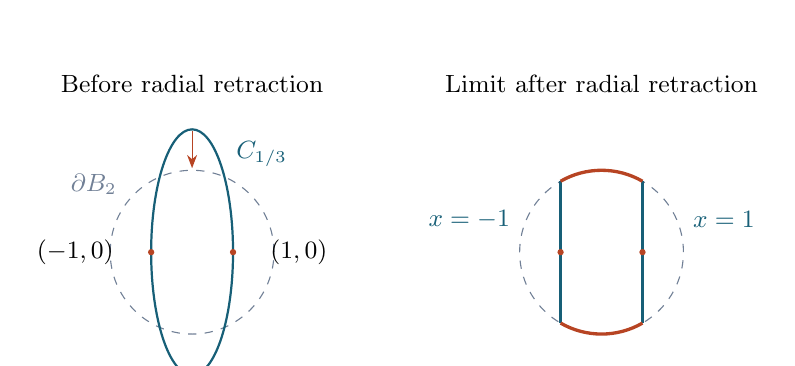
\begin{tikzpicture}[scale=0.52,font=\small]
\begin{scope}
\node at (0,4.1) {Before radial retraction};
\draw[curvegray,dashed] (0,0) circle (2);
\draw[curveblue,thick] (0,0) ellipse (1 and 3);
\draw[curvered,-{Stealth}] (0,2.95)--(0,2.05);
\node[curvegray] at (-2.4,1.65) {$\partial B_2$};
\node[curveblue] at (1.7,2.4) {$C_{1/3}$};
\fill[curvered] (-1,0) circle (2.2pt) node[left=10pt,black] {$(-1,0)$};
\fill[curvered] (1,0) circle (2.2pt) node[right=10pt,black] {$(1,0)$};
\end{scope}
\begin{scope}[xshift=10cm]
\node at (0,4.1) {Limit after radial retraction};
\draw[curvegray,dashed] (0,0) circle (2);
\draw[curveblue,thick] (-1,-1.7320508)--(-1,1.7320508);
\draw[curveblue,thick] (1,-1.7320508)--(1,1.7320508);
\draw[curvered,very thick] (60:2) arc (60:120:2);
\draw[curvered,very thick] (240:2) arc (240:300:2);
\fill[curvered] (-1,0) circle (2.2pt);
\fill[curvered] (1,0) circle (2.2pt);
\node[curveblue,left] at (-2,0.8) {$x=-1$};
\node[curveblue,right] at (2,0.8) {$x=1$};
\end{scope}
\end{tikzpicture}
\caption{The ellipses $x^2+\delta^2y^2=1$ contain both $(\pm1,0)$, whereas at $\delta=0$ the two points lie on different lines. In direction $\theta$, the retraction caps the radius $(\cos^2\theta+\delta^2\sin^2\theta)^{-1/2}$ at $2$. As $\delta\downarrow0$, the retracted sets converge to the two segments $x=\pm1$, $|y|\leq\sqrt3$, joined by the two arcs $x^2+y^2=4$, $|x|\leq1$. The arcs belong to the added circle factor.}
\end{figure}
Approximating any given labeled configuration by configurations from Lemma~\ref{lem:generic} and applying Lemma~\ref{lem:limit} proves the upper bound in \eqref{eq:main}. This argument also permits coincident limiting points.

\section{Optimizing the asymptotic coefficient}
Estimate~\eqref{eq:removal} retains more information than the inequality $q\geq k/2$ used for the uniform bound. For $0<a<\sqrt{2/37}$, choose $d=\lfloor a\sqrt m\rfloor$ at each sufficiently large stage. Apply Lemma~\ref{lem:generic} simultaneously through degree $\max(1,\lfloor a\sqrt n\rfloor)$. As $m\to\infty$,
\[
\frac km\longrightarrow\frac{a^2}2,\qquad
\frac{2(3d+1)^2}{m}\longrightarrow18a^2.
\]
It follows that $q/m\geq\beta(a)-o(1)$, uniformly over the point configurations, where
\begin{equation}\label{eq:beta}
\beta(a)=\frac{a^2}2\left(1-\frac{18a^2}{1-a^2/2}\right)>0.
\end{equation}
In particular, if $m'=m-q$, then
\[
\sqrt m-\sqrt{m'}\geq\sqrt m\left(1-\sqrt{1-\beta(a)+o(1)}\right).
\]
For each $C>L(a):=a/(1-\sqrt{1-\beta(a)})$, a threshold depending only on $a$ and $C$ therefore ensures that $d\leq C(\sqrt m-\sqrt{m'})$ at every stage above the threshold. The terminal cost and the circle cost in Lemma~\ref{lem:limit} are bounded independently of $n$. Summing, letting $n$ tend to infinity, and then letting $C$ decrease to $L(a)$ gives
\begin{equation}\label{eq:optimization}
\limsup_{n\to\infty}\frac{D(n)}{\sqrt n}
\leq\inf_{0<a<\sqrt{2/37}}\frac{a}{1-\sqrt{1-\beta(a)}}.
\end{equation}
Here are the details of the minimization. Put $x=a^2/2$, $y=x/(1-x)$, and $s=\sqrt{1-\beta}$. Then
\[
\beta=\frac{x(1-37x)}{1-x},\qquad
\beta-x\frac{d\beta}{dx}=36y^2,\qquad 0<y<1/36.
\]
At a stationary point of $\sqrt{2x}/(1-s)$, logarithmic differentiation gives $s(1-s)=x\,d\beta/dx$. Since $\beta=1-s^2$, this yields $1-s=36y^2$. Substituting $\beta=y(1-36y)/(1+y)$ and $s=1-36y^2$ gives
\begin{equation}\label{eq:root}
108y+72y^2-1296y^3-1296y^4=1.
\end{equation}
The derivative of the left-hand side is $108+144y-3888y^2-5184y^3>104$ on $(0,1/36)$. The objective tends to infinity at both endpoints of the interval, so its minimum occurs at its unique stationary point. The root of \eqref{eq:root} is approximately $0.00921215119$, giving $a\approx0.135115226$ and $L(a)\approx44.22620514$.

For an exact check of the strict bound in Theorem~\ref{thm:strong}, take $a=27/200$ and $c=4423/100$. Substitution in \eqref{eq:beta} gives $\beta(a)>2a/c-(a/c)^2$, hence $L(a)<c$. These bounds do not determine whether $D(n)/\sqrt n$ has a limit.

\begin{thebibliography}{9}
\bibitem{dk1} A. Degtyarev and V. Kharlamov, \emph{Topological properties of real algebraic varieties: du c\^ot\'e de chez Rokhlin}, Russian Math. Surveys \textbf{55} (2000), 735--814. \href{https://arxiv.org/abs/math/0004134}{arXiv:math/0004134}.
\bibitem{fulton} W. Fulton, \emph{Algebraic Curves: An Introduction to Algebraic Geometry}, W. A. Benjamin, 1969. Author's electronic edition.
\bibitem{sard} A. Sard, \emph{The measure of the critical values of differentiable maps}, Bull. Amer. Math. Soc. \textbf{48} (1942), 883--890. \href{https://doi.org/10.1090/S0002-9904-1942-07811-6}{doi:10.1090/S0002-9904-1942-07811-6}.
\end{thebibliography}
\noindent\textbf{Curator affiliations}\par
Paata Ivanisvili, Department of Mathematics, University of California, Irvine.\par
Aleksandr Logunov, Department of Mathematics, Massachusetts Institute of Technology.
\end{document}
